\chapter{DATA C100: Gradient Descent}

\section{Computational Minimization of Loss Function}
We have been able to minimize the loss functions provided for prior linear regression models. But we may always encounter harder loss functions to analyze, either via calculus or linear algebra-geometry. \\
This is where we fall back to the power of computation. Numerical computing. Such subfield of computer science focuses on solving complex mathematical problems using arithmetic operations. Very fortunately, Python is well supported by such libraries:
\setbox\codebox=\hbox{
    \begin{lstlisting}
    scipy.optimize.minimize
    Args:
        fun: The objective function to be minimized, where $x$ is a 1D
        array.
        x0: Initial guess, with the same size as input x from fun.
    Returns:
        The result of optimization with a solution array for optimal
        parameters.
    Example:
        >>> from scipy.optimize import minimize
        >>> minimize(arbitrary, x0 = [6, 3])
        OptimizationResult(x = [5.5, 2])
    \end{lstlisting}
}
\begin{ln-code}{Using scipy to Minimize Functions}{}
    \usebox\codebox
\end{ln-code}

\section{Gradient Descent Algorithm}
When in a multivariable context, the loss function might take plural inputs and thus not be plottable in the two-dimensional space anymore. In that case, each point $(x_1, x_2)$ correspond to the cost of choosing them as model parameters, and we end up with a loss surface.
\begin{ln-fig}{Loss Function as a Surface}{}
    \begin{center}
        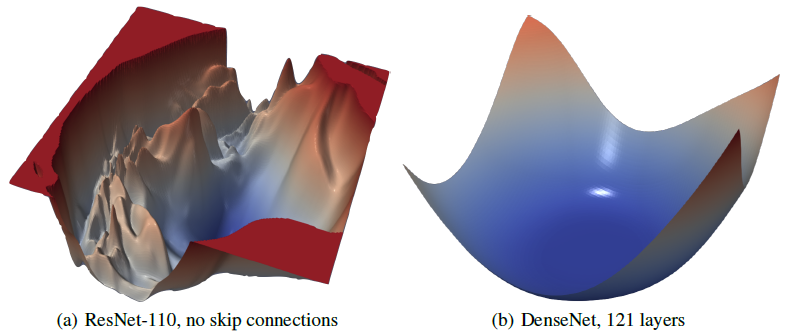
\includegraphics[scale=0.4]{figs/ln04/loss-surface.png}
    \end{center}
    As you may see, each point $(x_1, x_2)$ has a respective height for their respective loss value. Therefore, the lowest point on the surface is the point of optimization, where by choosing that point as the set of parameters, we arrive at the lowest possible loss value. \\
    We will also take notice on why the right-side surface is much preferrable than the left-side surface.
\end{ln-fig}
Now, our task is focused on ``how to descend on the loss surface''. The entire algorithm that breifly leads us to descend off the loss surface is therefore known as the Gradient Descent Algorithm.

\subsection{Interpretation of Gradients}
This section is noted from MATH 53. It is not in scope for DATA C100. However, I think the reader can benefit from knowing what gradients are. I also consider writing a section for gradients if I have the fortune of addressing MATH 53 in this writing. \\
Let us begin with the notion of Directional Derivatives:
\begin{ln-define}{Directional Derivatives}{}
    We know how to compute the partial derivatives for a function $f(x, y)$ with respect to $x$ and $y$, which are respectively the rate of change of $f$ as we solely vary $x$ and solely vary $y$. \\
    The \textbf{directional derivative}, then, is the rate of change of $f$ when we let both variables $x$ and $y$ change. Mathematically, we would be able to characterize the direction of changing as a vector. \\
    The rate of change of $f(x, y)$ along a unit vector $\vec{u} = \langle a, b \rangle$ can thus be denoted as:
    \[D_{\vec{u}}f(x, y) = \lim_{h \rightarrow 0} \frac{f(x + ah, y + bh) - f(x, y)}{h}\]
    In practical form, after a series of derivations:
    \[D_{\vec{u}}f(x, y) = \langle f_x (x, y), f_y (x, y) \rangle \cdot \vec{u}\]
\end{ln-define}
Recall that:
\[\cos(\theta_{\vec{u}, \vec{v}}) = \frac{\vec{u} \cdot \vec{v}}{|\vec{u}| |\vec{v}|}\]
Therefore, the directional derivative is maximized when the direction at which we change $x$ and $y$ is exactly the vector $\langle f_x (x, y), f_y (x, y) \rangle$. \\
This means the direction provides the most positive change (provides the maximal rate of change) towards $f$, if we were to travel in that direction. For convenience and mathematical property, let us name this great observation as follows:
\begin{ln-define}{Gradient}{}
    The \textbf{gradient} of a function $f(x_1, \cdots, x_n)$ is the vector:
    \[\nabla f = \begin{bmatrix} \pdv{f}{x_1} \\ \cdots \\ \pdv{f}{x_n} \end{bmatrix}\]
    Where $\nabla f(x_1, \cdots, x_n)$ notes the direction of greatest ascent (greatest rate of value increase) along the function $f$ from $(x_1, \cdots, x_n)$
\end{ln-define}
This brings an implication: the opposite direction of the gradient is the direction of greatest descent. We can thus come up with the following iterative procedure for descending along a loss surface of $f(x, y)$:
\setbox\codebox=\hbox{
    \begin{lstlisting}
    initial_guess = ? #an array of parameters for initial guess
    for _ in range(epoch):
        grad = gradient(f, x, y)
        initial_guess -= grad
    return initial_guess
    \end{lstlisting}
}
\begin{ln-code}{Sketch of Gradient Descent Algorithm}{}
    \usebox\codebox
\end{ln-code}
As a side note of interest, COMPSCI 61A used to cover a two-dimensional version of gradient descent to discuss the work of `iteration' in computer science.

\subsection{Improving the Gradient Descent Sketch}
We have a few problems left. \\
First of all:
\begin{center}
    What if the direction of greatest descent doesn't lead us down anymore?
\end{center}
For example:
\begin{ln-fig}[sidebyside]{Divergence of Gradient Descent}{}
    \begin{center}
        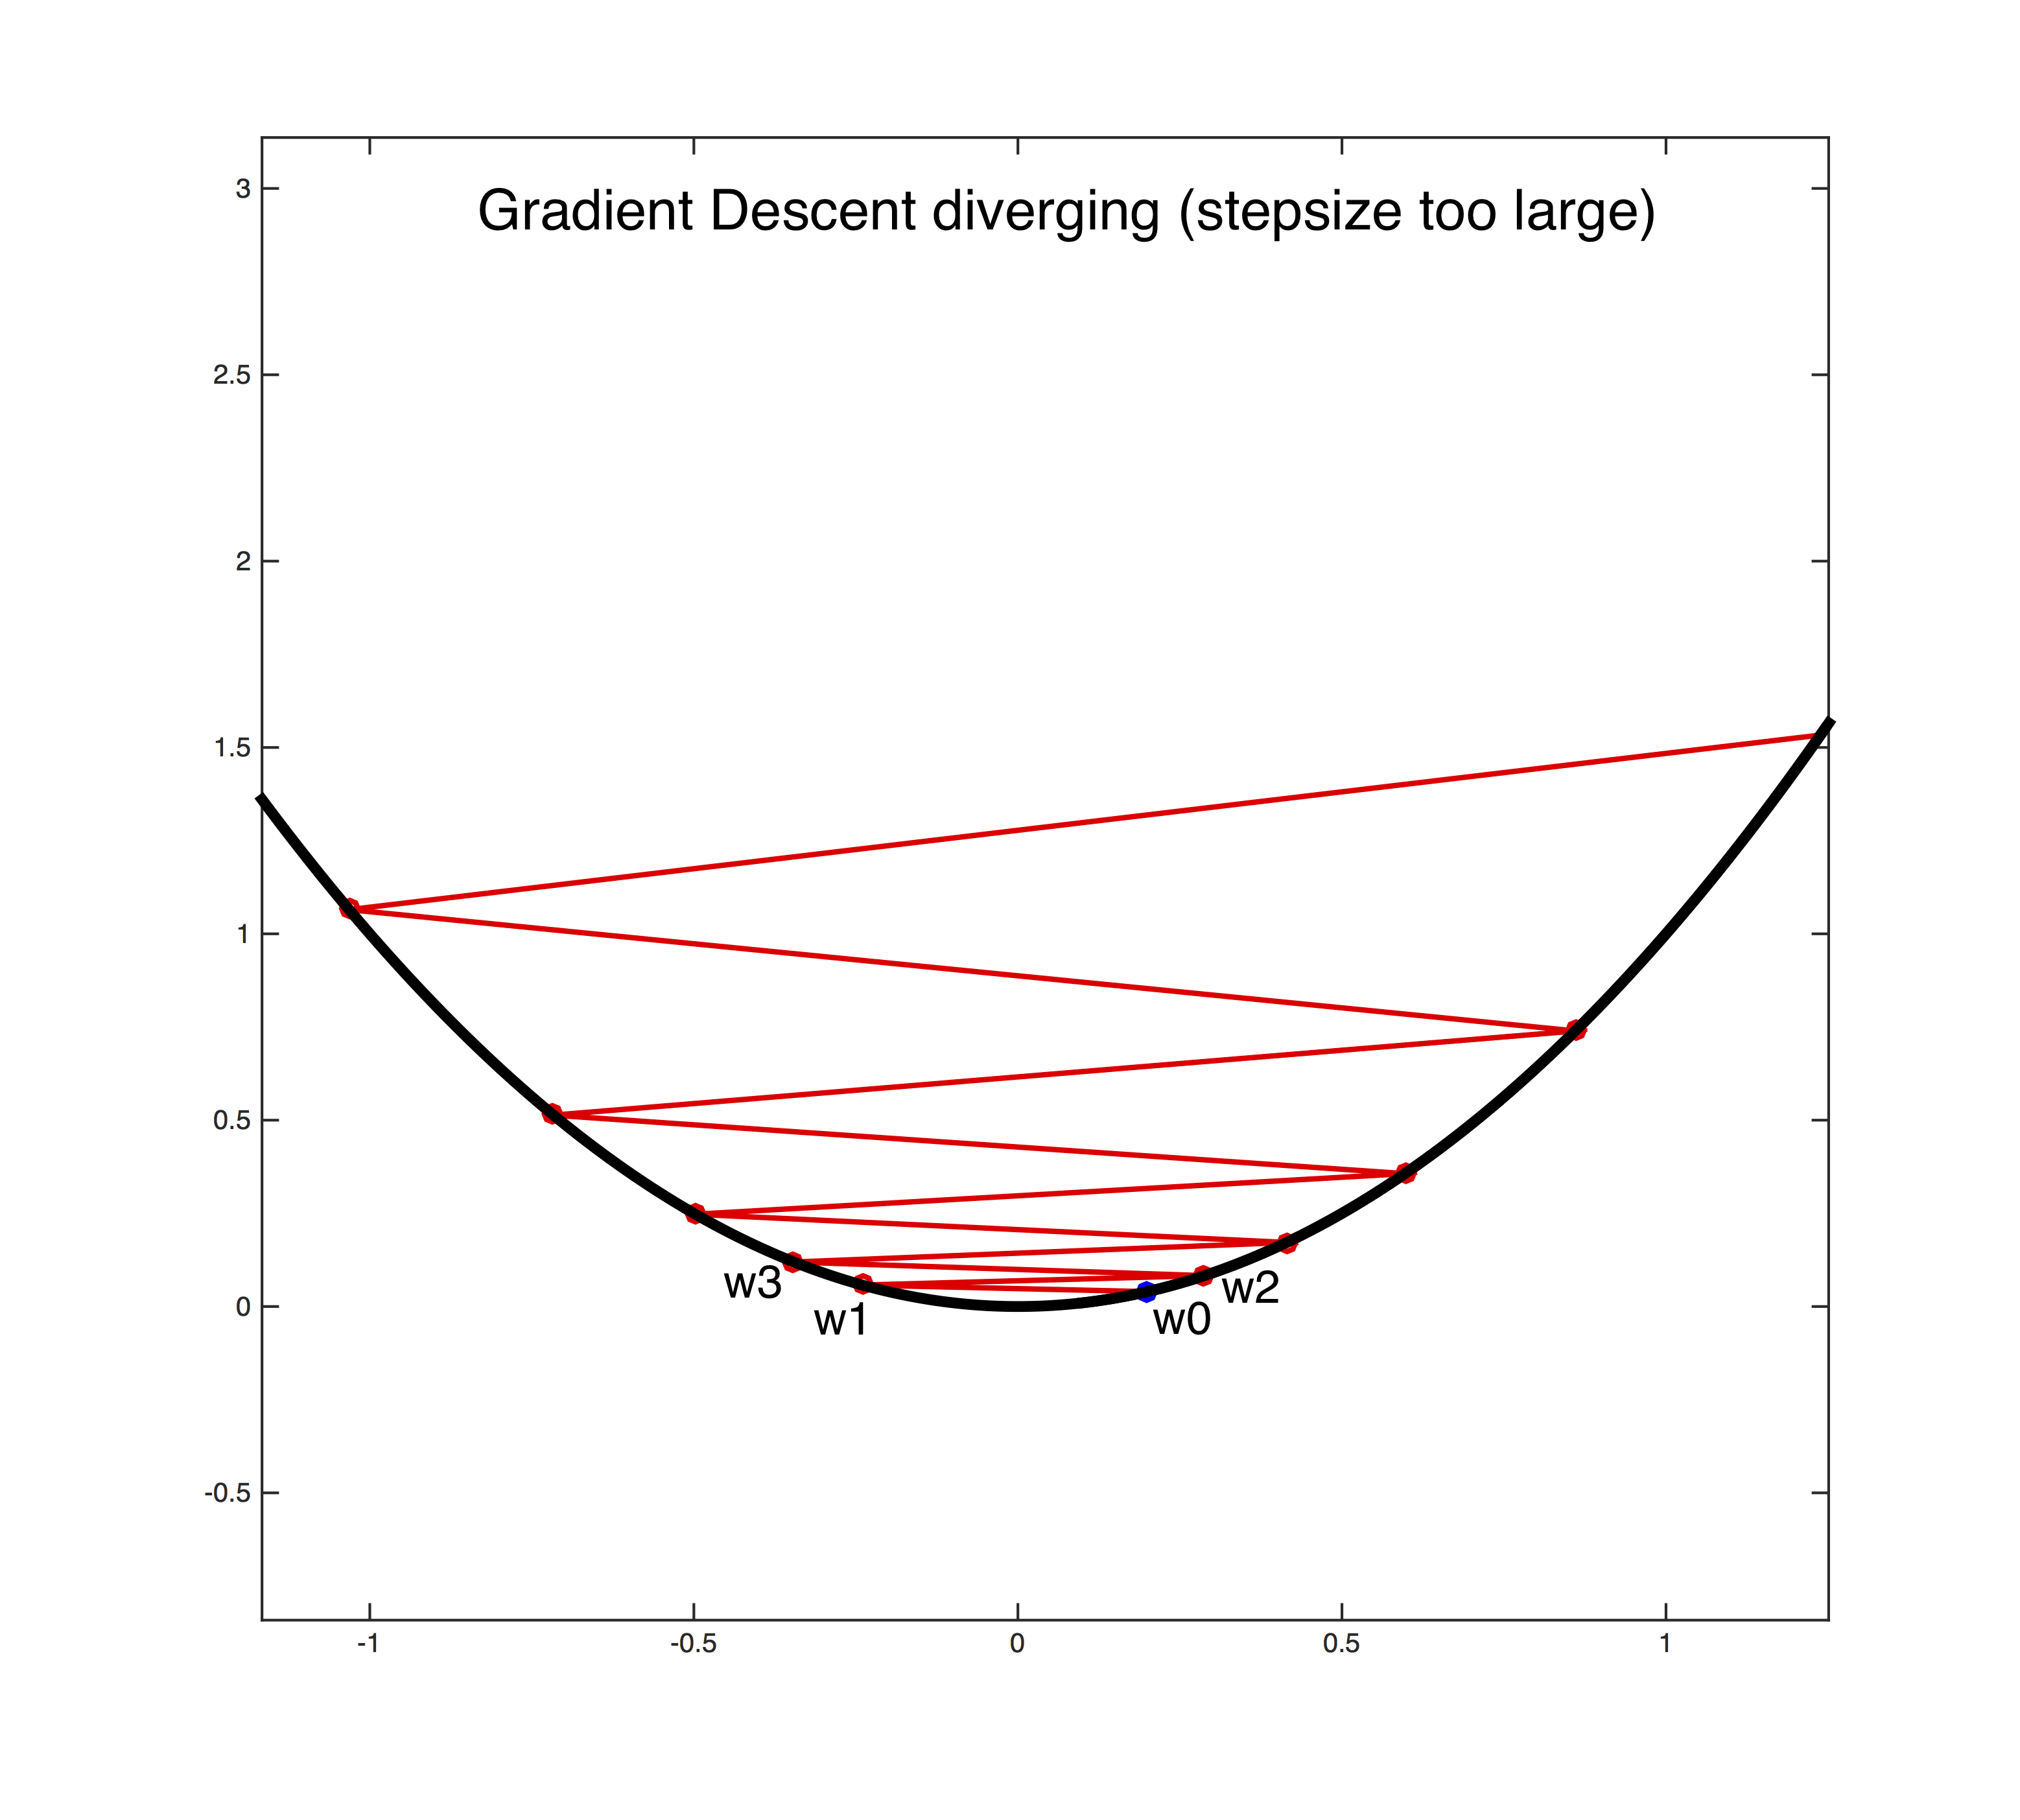
\includegraphics[scale=0.25]{figs/ln04/grad-descent-diverge.png}
    \end{center}
    \tcblower
    As you may see, because the gradient's magnitude is too big, we ended up going away from the local minima. \\
    To correct this situation, we will now improve the sketch of gradient algorithm to involve a parameter that controls what portion of the gradient do we travel. We call this the \textbf{learning step} ($\alpha$).
\end{ln-fig}
However, notice that if the learning step is small, then the distance at which we descent along the loss surface would also be smaller per iteration. This makes it take too long for gradient descent to converge at the minimum. 
Therefore, we would usually need to try learning steps by increasing or decreasing it tenfold until we find the appropriate learning step, and perhaps make it smaller as we go onto further iterations:
\setbox\codebox=\hbox{
    \begin{lstlisting}
    alpha = ? $customized learning step
    initial_guess = ? #an array of parameters for initial guess
    for _ in range(epoch):
        grad = gradient(f, x, y)
        initial_guess -= alpha * grad
    return initial_guess
    \end{lstlisting}
}
\begin{ln-code}{Gradient Descent Algorithm}{}
    \usebox\codebox \\
    Mathematically expressed as a state-transition system (borrowing the insights and works of EECS 16A):
    \[\vec{\theta}[t + 1] = \vec{\theta}[t] - a \nabla L(\vec{\theta}, x_1, \cdots, x_n)\]
\end{ln-code}

\subsection{Convexity}
We still have not decided how to make an initial guess of parameters, as well as how does gradient descent behave in real life. \\
First of all, let's perform a thought experiment. Suppose our loss function is a curve along which we gradient descent, what happens when we set the initial guess to the left side of the curve, and what happens when we guess from the right side of the curve instead?
\begin{ln-fig}[]{Loss Functions with Local Minima}{}
    \begin{center}
        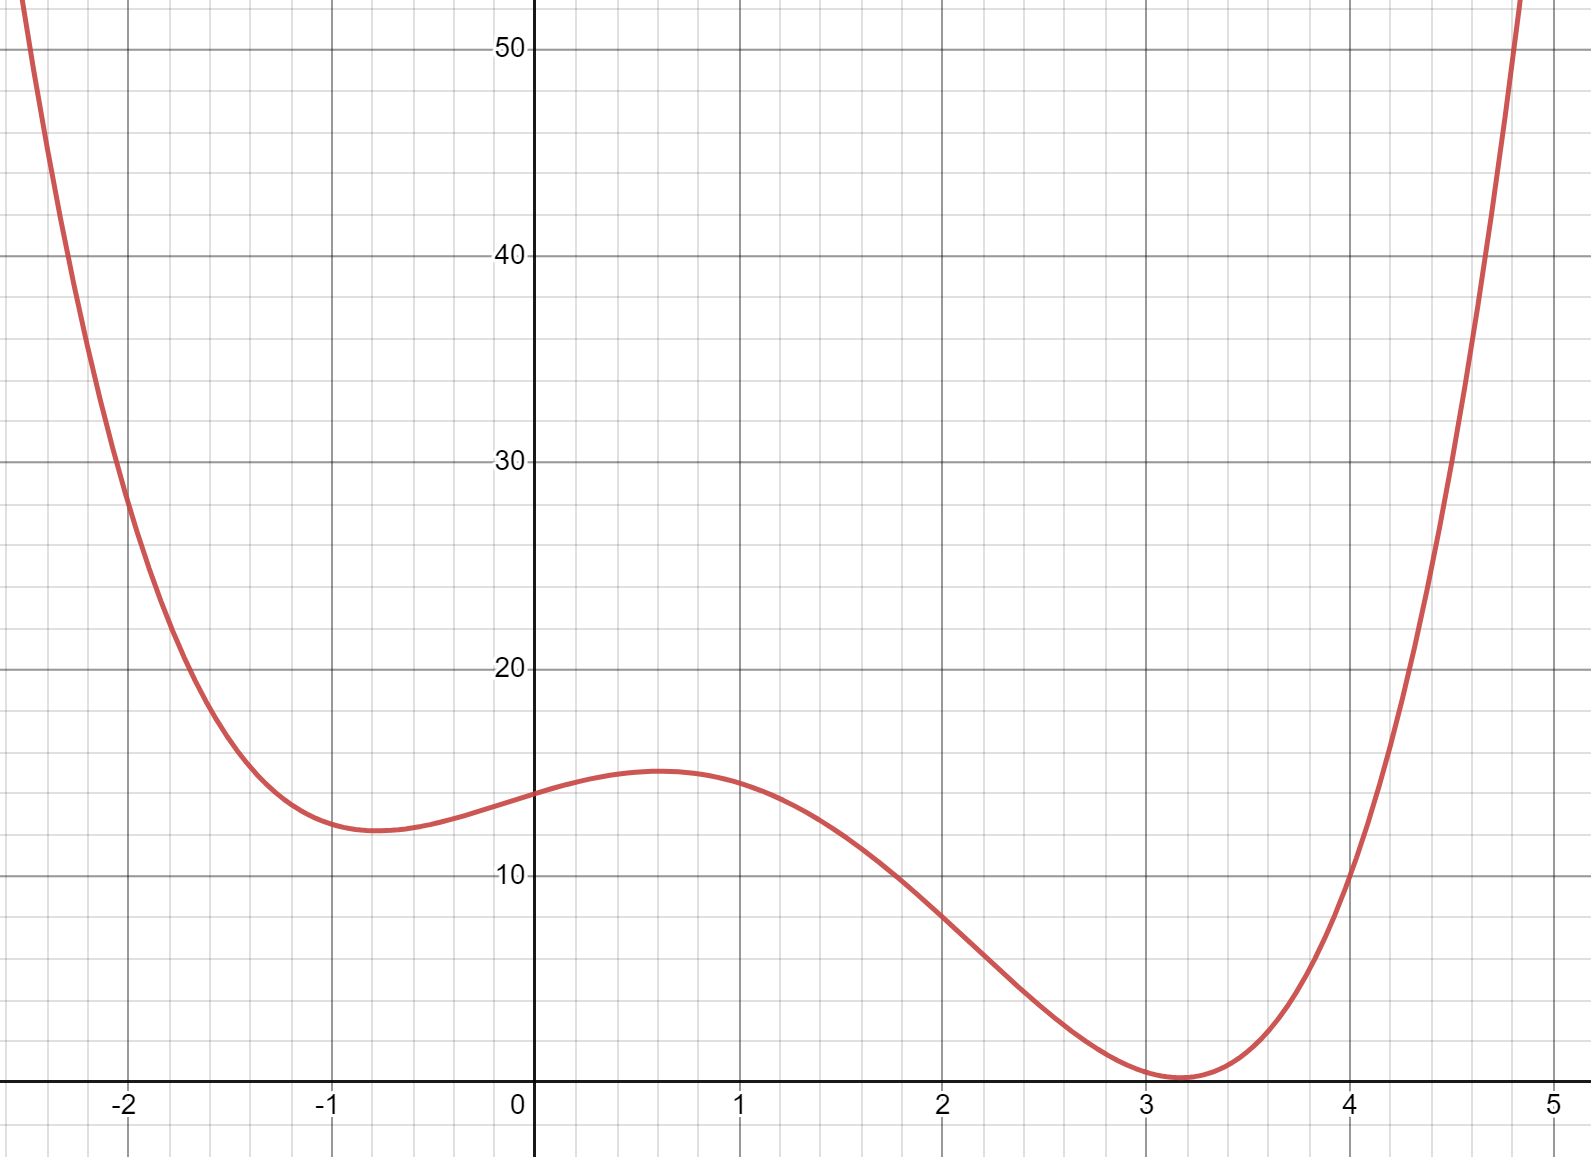
\includegraphics[scale=0.3]{figs/ln04/several-local-min.png}
    \end{center}
\end{ln-fig}
In this case, guessing from different directions would lead us to different local minima. Therefore, it is not exactly guaranteed that gradient descent leads us to the global minimum of our loss surface. \\
Then, if we manage to compromise with that (which we would have to, for now), how do we initialize our guess? This is where the idea of random initialization comes in for more complex models, where, we initialize each parameter to a random number as our initial guess. \\
For the scope of DATA C100, we would stick with zero initialization, where the initial guess of parameters would all be $0$. This would lead to a problem. If the gradient descent updates unfortunately lead to the parameters keep being equal, then we will realistically make no improvements on the model since every predictor variable receives the same weight in a regression equation. But, for now, let us not worry about this until a long time later.

But some functions guarantee us to find a global minimum when using gradient descent. These functions are called \textbf{convex functions}:
\begin{ln-define}{Convexity}{}
    Function $f$ is convex iff:
    \[\forall a, b \in D_f, t \in [0, 1] (tf(a) + (1 - t)f(b) \geq f(ta + (1 - t)b))\]
    Or in English: if a line is drawn between two points on the curve, all values on the curve must be on or below the line.
\end{ln-define}

\subsection{Stochastic Gradient Descent}
Sometimes, our dataset is too big. We would therefore need to perform gradient descent by batches:
\begin{ln-define}{Mini-Batch Gradient Descent}{}
    In mini-batch gradient descent, we use a subset of data to calculate the gradient. \\
    An approximate sketch of procedure follows:
    \begin{bindenum}
        \item Decide a batch size (The amount of data used to compute gradient). A popular choice is 32 (according to professor, for no particular reason it seems).
        \item For all batches:
        \subitem Compute gradient on current batch of the data
        \item Repeat the process until we arrive at a stopping condition where we decide we have optimized the parameters sufficiently.
    \end{bindenum}
\end{ln-define}
Via mini-batch gradient descent, we avoid heavy computational costs for large datasets and in turn are provided an approximation of the best way down an approximately true loss surface. It works well enough in practice.

We can also choose a batch size of $1$, which would be a process called \textbf{Stochastic Gradient Descent} (SGD in some libraries). \\
In this case, we compute gradient based on one single data point. This technique is used on datasets whose data entries involve many parameters, as via one datapoint, we may have updated millions of parameters for that epoch. In the long run, the effect of SGD is very similar to computing the true gradient based on the entire dataset. Therefore, it is also a practice-able choice for real-life machine learning models.
